\section*{Kapitel 7 - Fortgeschrittenere lineare Modelle}

\begin{multicols*}{3}

\tikzstyle{mybox} = [draw=black, fill=white, very thick,
    rectangle, rounded corners, inner sep=10pt, inner ysep=10pt]
\tikzstyle{fancytitle} =[fill=black, text=white, font=\bfseries]



%------------ Das Allgemeine lineare Regressionsmodell ---------------
\begin{tikzpicture}
    \node [mybox] (box){
    \begin{minipage}{0.3\textwidth}
    Das \tc{allgemeine lineare Regressionsmodell} hat die Form
    $$\bY = \bX\bbeta + \beps,$$ wobei wir nun annehmen, dass $\beps \sim
    \Ncal(\bf0, \ssd \bW^{-1})$, mit \textbf{bekannter} positiv definiter Matrix $\bW$. Wir nennen
    $\bW$ die \tc{Gewichtsmatrix}.

    Im Falle von heteroskedastischen, aber unkorrelierten Fehlern ist $\bW$ eine
    Diagonalmatrix mit $\bW = \diag(w_1, \cdots, w_n)$ und $\V(\beps) = 
    \diag(\frac{\ssd}{w_1}, \cdots, \frac{\ssd}{w_n})$.
    \end{minipage}
    };
%------------ Das Allgemeine lineare Regressionsmodell Header ---------------------
\node[fill = black, text=white, font=\bfseries, right=10pt] at (box.north west) 
{Das allgemeine lineare Regressionsmodell};
\end{tikzpicture}

%------------ Schätzer im allgemeinen lineare Regressionsmodell ---------------
\begin{tikzpicture}
    \node [mybox] (box){
    \begin{minipage}{0.3\textwidth}
    Gegeben sei das \tc{allgemeine lineare Regressionsmodell}
    $\bY = \bX\bbeta + \beps$ mit $\beps \sim \Ncal(\bf0, \ssd \bW^{-1})$.

    Dann gilt:
    \begin{align*}
        \hbbeta &= (\bX^\top\bW\bX)^{-1}\bX^\top\bW\bY,\\
        \E(\hbbeta) &= \bbeta,\\
        \V(\hbbeta) &= \ssd(\bX^\top\bW\bX)^{-1}
    \end{align*}
    und $\hbbeta$ ist der \tc{Beste lineare unverzerrte Schätzer} (BLUE) für $\bbeta$.
    
    Der \tc{Schätzer für $\ssd$} ist gegeben durch den REML-Schätzer
    $$\hssd = \frac{\hbeps^\top \bW \hbeps}{n - p'},$$

    \tc{!} Alle Schätzer setzen voraus, dass $\bW$ bekannt ist.

    \end{minipage}
    };
%------------ Schätzer im allgemeinen lineare Regressionsmodell Header ---------------------
\node[fill = purple, text=white, font=\bfseries, right=10pt] at (box.north west) 
{Schätzer im allg. linearen Regressionsmodell};
\end{tikzpicture}

%------------ Umformung ---------------
\begin{tikzpicture}
    \node [mybox] (box){
    \begin{minipage}{0.3\textwidth}
    Wir können die symmetrische positiv definite Gewichtsmatrix $\bW$
    zerlegen durch $$\bW = \bV\bD\bV^\top,$$ wobei $\bD$ eine Diagonalmatrix
    ist.
    Dann definieren wir $\bW^{\frac{1}{2}} = \bV\bD^{\frac{1}{2}}\bV^\top$.
    Mit dieser Zerlegung können wir das allgemeine lineare Regressionsmodell
    in ein klassisches lineares Regressionsmodell umformen durch
    $$\bY^* = \bX^*\bbeta^* + \beps^*, \quad \beps^* \sim \Ncal(\bf0, \ssd \bI)$$ wobei
    $$\bY^* = \bW^{\frac{1}{2}}\bY, \quad \bX^* = \bW^{\frac{1}{2}}\bX, \quad
    \beps^* = \bW^{\frac{1}{2}}\beps.$$

    \end{minipage}
    };
%------------ Umformung Header ---------------------
\node[fill = purple, text=white, font=\bfseries, right=10pt] at (box.north west) 
{Umformung};
\end{tikzpicture}

%------------ AR(1) Modell ---------------
\begin{tikzpicture}
    \node [mybox] (box){
    \begin{minipage}{0.3\textwidth}
    
    Das \tc{AR(1) Zeitreihenmodell} hat die Form
    $$\eps_t = \phi \eps_{t-1} + \eta_t, \quad t = 2,\dots,n$$ wobei $\eta_t
    \sim \Ncal(0, \sigma^2), |\phi| < 1$ und $\V(\eps_1) = \frac{\ssd}{1-\phi^2}$.

    Dann ist die Kovarianzmatrix $\bW^{-1}$ gegeben durch
    $$\bW^{-1} = \frac{1}{1 - \phi^2} \begin{pmatrix}
        1 & \phi & \phi^2 & \cdots & \phi^{n-1}\\
        \phi & 1 & \phi & \cdots & \phi^{n-2}\\
        \phi^2 & \phi & 1 & \cdots & \phi^{n-3}\\
        \vdots & \vdots & \vdots & \ddots & \vdots\\
        \phi^{n-1} & \phi^{n-2} & \phi^{n-3} & \cdots & 1
    \end{pmatrix}$$
    Damit gilt also
    $$\beps \sim \Ncal(\bf0, \ssd \bW^{-1}).$$

    \end{minipage}
    };
%------------ AR(1) Header ---------------------
\node[fill = blue, text=white, font=\bfseries, right=10pt] at (box.north west) 
{AR(1) Zeitreihenmodell};
\end{tikzpicture}

%------------ Linear Mixed Modell ---------------
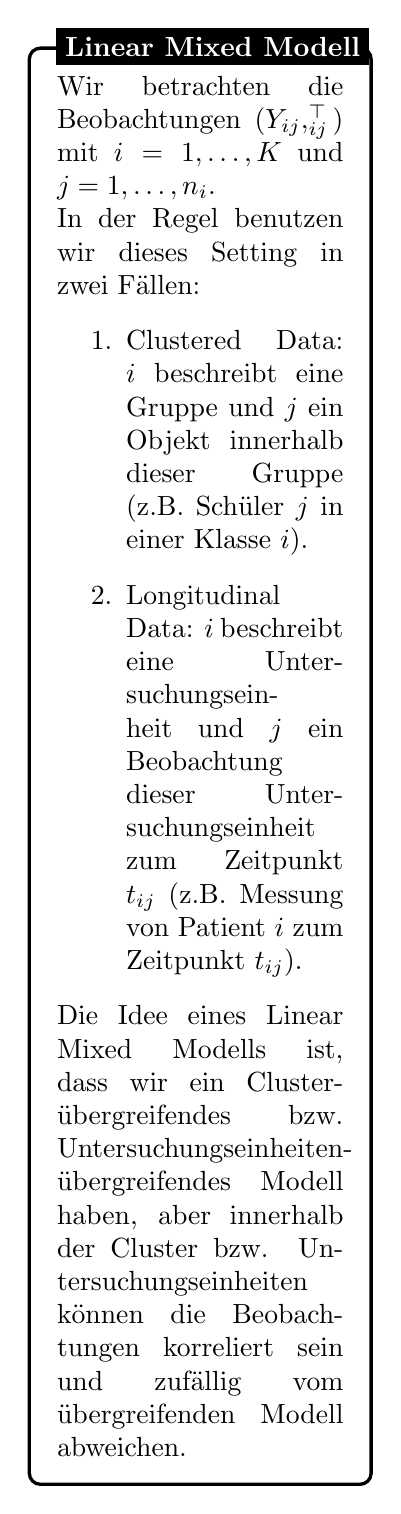
\begin{tikzpicture}
    \node [mybox] (box){
    \begin{minipage}{0.3\textwidth}

    Wir betrachten die Beobachtungen $(Y_{ij}, \bx_{ij}^\top)$ mit $i =
    1,\dots,K$ und $j = 1,\dots,n_i$.
    
    In der Regel benutzen wir dieses Setting in zwei Fällen:
    \begin{enumerate}
        \item Clustered Data: $i$ beschreibt eine Gruppe und $j$ ein Objekt
        innerhalb dieser Gruppe (z.B. Schüler $j$ in einer Klasse $i$).
        \item Longitudinal Data: $i$ beschreibt eine Untersuchungseinheit und
        $j$ ein Beobachtung dieser Untersuchungseinheit zum Zeitpunkt $t_{ij}$
        (z.B. Messung von Patient $i$ zum Zeitpunkt $t_{ij}$).
    \end{enumerate}
    
    Die Idee eines \tc{Linear Mixed Modells} ist, dass wir ein Cluster-übergreifendes
    bzw. Untersuchungseinheiten-übergreifendes Modell haben, aber innerhalb der
    Cluster bzw. Untersuchungseinheiten können die Beobachtungen korreliert sein und
    zufällig vom übergreifenden Modell abweichen.

    
\end{minipage}
};
%------------ Linear Mixed Modell Header ---------------------
\node[fill = black, text=white, font=\bfseries, right=10pt] at (box.north west) 
{Linear Mixed Modell};
\end{tikzpicture}

%------------ Linear Mixed Modell ---------------
\begin{tikzpicture}
    \node [mybox] (box){
    \begin{minipage}{0.3\textwidth}

    Das \tc{Random Intercept Modell} ist definert durch
    $$Y_{ij} = \bx_{ij}^\top\bbeta + \gamma_{0i} + \eps_{ij}, \quad i =
    1,\dots,K, \quad j = 1,\dots,n_i$$ mit $\eps_{ij} \sim \Ncal(0,\ssd),
    i.i.d.$ und $\gamma_{0i} \sim \Ncal(0, \ssd_{\gamma_0}), i.i.d.$ und
    $\sum_{i = 1}^{K} n_i = n$ und der Annahme, dass die $\eps_{ij}$ unabhängig
    von den $\gamma_{0i}$ sind.\\

    Wir bezeichnen $\beta_0$ als den fixed Population Intercept und
    $\gamma_{0i}$ als die Cluster-spezifische bzw.
    Untersuchungseinheiten-spezifische zufällige Abweichung vom fixed Population
    Intercept. Zusammen bezeichnen wir $\beta_0 + \gamma_{0i}$ als den
    \tc{random Intercept} von Cluster/Untersuchungseinheit $i$. Die restlichen
    $\beta_j$ sind die \tc{fixed Effekte}.\\

    Zwischen den Cluster/Untersuchungseinheiten sind die $Y_{ij}$ unabhängig
    und es gilt das konditionalle Modell für $i = 1,\dots,K$
    $$Y_{ij}\mid \gamma_{0i} \sim \Ncal(\bx_{ij}^\top\bbeta + \gamma_{0i},
    \ssd).$$

    Innerhalb eines Clusters/Untersuchungseinheit sind die $Y_{ij}$ korreliert.
    Wir bezeichnen diese Korrelation als \tc{Intra-Class Correlation} (ICC). Es gilt
    $$\corr(Y_{ij}, Y_{il})= \frac{\ssd_{\gamma_0}}{\ssd_{\gamma_0} + \ssd}, \quad j,l = 1,\dots,n_i, j\neq l$$
    und
    $$\V(\bY_i) = \ssd\bI_{n_i} + \ssd_{\gamma_0} \bJ_{n_i}, \quad i = 1,\dots,K$$
    wobei $\bJ_{n_i}$ die $n_i \times n_i$-Matrix mit Einsen ist.

    Daraus ergibt sich das \tc{marginale Modell}
    $$\bY_i \sim \Ncal(\bX_i\bbeta, \ssd\bI_{n_i} + \ssd_{\gamma_0} \bJ_{n_i}).$$

    \tc{!} Bei dem Random Intercept Modell wird die
    Annahme gemacht, dass die Effekte von $x$ auf $Y$ innerhalb
    der Cluster/UEs und über diese hinweg gleich sind. Das kann
    zu falschen Schlüssen führen, wenn diese Annahme nicht zutrifft (z.B. Simpson's Paradoxon).
    Eine Möglichkeit das zu korrigieren, ist das erweiterte Random Intercept Modell.
    $$Y_{ij} = \beta_0 + \beta_1(x_{ij} - \bar{x}_i) + \beta_2 \bar{x}_i + \gamma_{0i} + \eps_{ij}$$

    \end{minipage}
    };
%------------ Linear Mixed Modell Header ---------------------
\node[fill = black, text=white, font=\bfseries, right=10pt] at (box.north west) 
{Random Intercept Modell};
\end{tikzpicture}

%------------ Logistisches Regressionsmodell ---------------
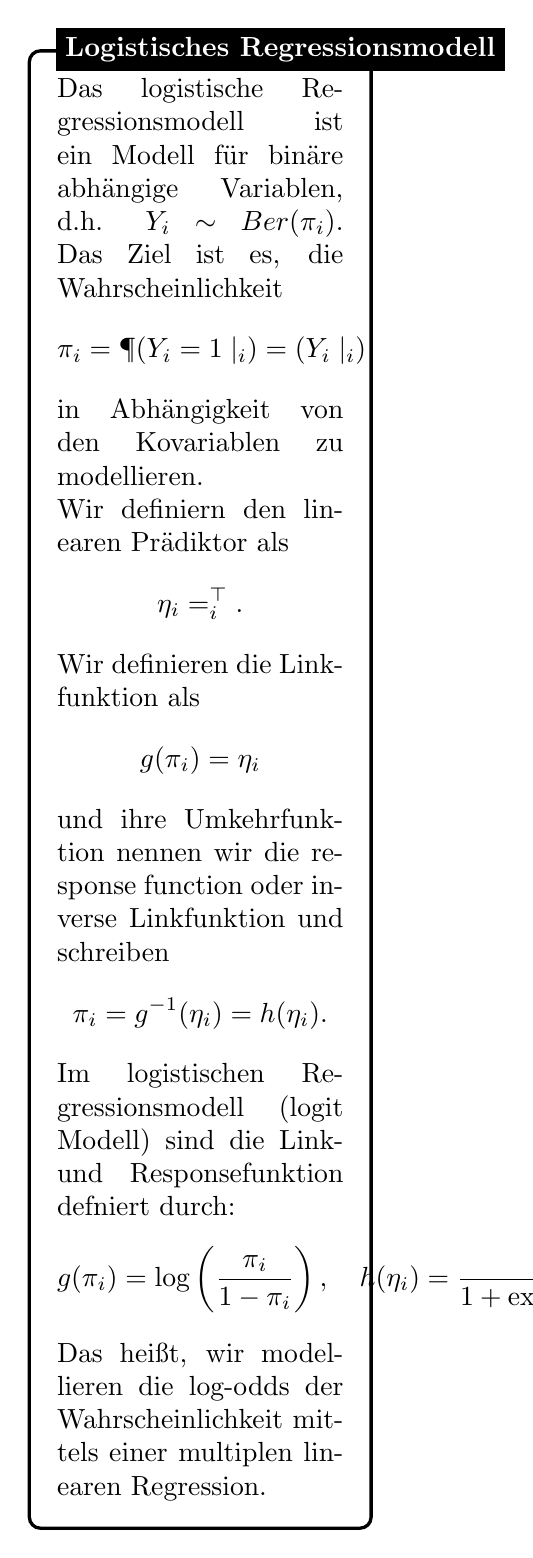
\begin{tikzpicture}
    \node [mybox] (box){
    \begin{minipage}{0.3\textwidth}
    
    Das \tc{logistische Regressionsmodell} ist ein Modell für binäre
    abhängige Variablen, d.h. $Y_i \sim Ber(\pi_i)$. Das Ziel ist es, die Wahrscheinlichkeit
    $$\pi_i = \P(Y_i = 1 \mid \bx_i) = \E(Y_i\mid \bx_i)$$ 
    in Abhängigkeit von den Kovariablen zu modellieren.

    Wir definiern den \tc{linearen Prädiktor} als
    $$\eta_i = \bx_i^\top\bbeta.$$
    Wir definieren die \tc{Linkfunktion} als
    $$g(\pi_i) = \eta_i$$ und ihre Umkehrfunktion nennen wir die
    \tc{response function} oder \tc{inverse Linkfunktion} und schreiben
    $$\pi_i = g^{-1}(\eta_i) = h(\eta_i).$$

    Im \tc{logistischen Regressionsmodell (logit Modell)} sind die Link- und
    Responsefunktion defniert durch:
    $$g(\pi_i) = \log\left(\frac{\pi_i}{1 - \pi_i}\right), \quad
    h(\eta_i) = \frac{1}{1 + \exp(-\eta_i)}.$$
    Das heißt, wir modellieren die log-odds der Wahrscheinlichkeit mittels einer
    multiplen linearen Regression.
    \end{minipage}
    };
%------------ Logistisches Regressionsmodell Header ---------------------
\node[fill = black, text=white, font=\bfseries, right=10pt] at (box.north west) 
{Logistisches Regressionsmodell};
\end{tikzpicture}

%------------ Interpretation Logistisches Regressionsmodell ---------------
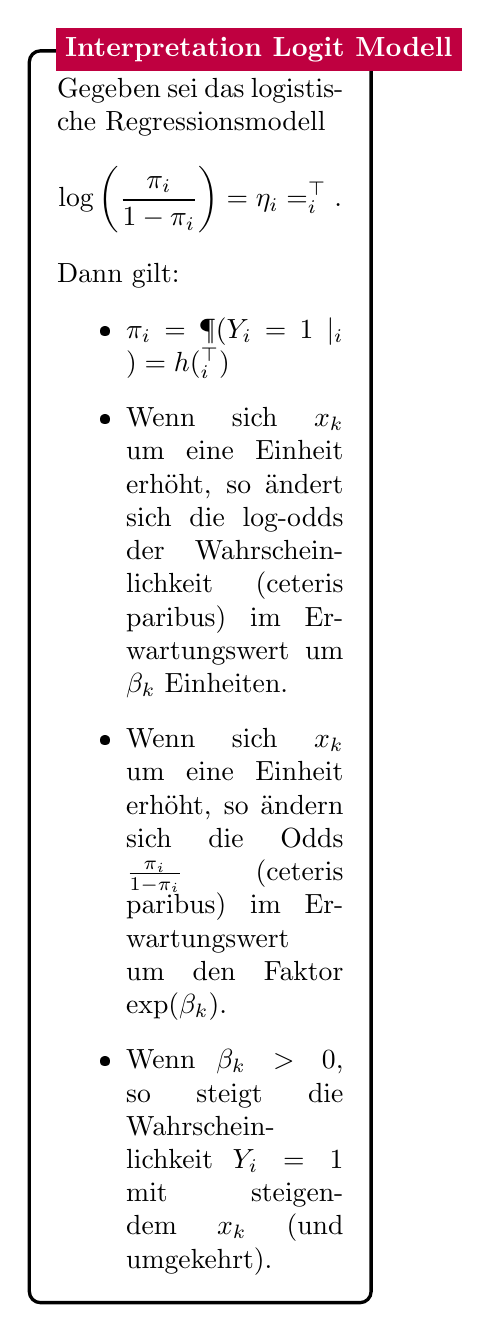
\begin{tikzpicture}
    \node [mybox] (box){
    \begin{minipage}{0.3\textwidth}
    
    Gegeben sei das \tc{logistische Regressionsmodell}
    $$\log\left(\frac{\pi_i}{1 - \pi_i}\right) = \eta_i = \bx_i^\top\bbeta.$$

    Dann gilt:
    \begin{itemize}
        \item $\pi_i = \P(Y_i = 1 \mid \bx_i) = h(\bx_i^\top\bbeta)$
        \item Wenn sich $x_k$ um eine Einheit erhöht, so ändert sich die
        log-odds der Wahrscheinlichkeit (ceteris paribus) im Erwartungswert um
        $\beta_k$ Einheiten.
        \item Wenn sich $x_k$ um eine Einheit erhöht, so ändern sich die Odds
        $\frac{\pi_i}{1 - \pi_i}$ (ceteris paribus) im Erwartungswert um den
        Faktor $\exp(\beta_k)$.
        \item Wenn $\beta_k > 0$, so steigt die Wahrscheinlichkeit $Y_i = 1$ mit
        steigendem $x_k$ (und umgekehrt).
        
    \end{itemize}
    
    \end{minipage}
    };
%------------ Interpretation Logistisches Regressionsmodell Header ---------------------
\node[fill = purple, text=white, font=\bfseries, right=10pt] at (box.north west) 
{Interpretation Logit Modell};
\end{tikzpicture}

%------------ Logit Modell in R ---------------
\begin{tikzpicture}
    \node [mybox] (box){
    \begin{minipage}{0.3\textwidth}
    
    In R können wir ein logistisches Regressionsmodell mit der Funktion
    \texttt{glm()} schätzen. Die Syntax ist
    \begin{lstlisting}
    glm(Y ~ X1 + X2 + ..., data = data,
    family = binomial(link = "logit"))
    \end{lstlisting}
    wobei \texttt{Y} die abhängige Variable und \texttt{X1, X2, ...} die
    unabhängigen Variablen sind.

    \end{minipage}
    };
%------------ Logit Modell in R Header ---------------------
\node[fill = olive, text=white, font=\bfseries, right=10pt] at (box.north west) 
{Logit Modell in R};
\end{tikzpicture}

%------------ MLE ---------------
\begin{tikzpicture}
    \node [mybox] (box){
    \begin{minipage}{0.3\textwidth}
    
    Die log-likelihood Funktion lautet
    $$\ell(\bbeta) = \sum_{i = 1}^{n} y_i\log(\pi_i) + (1 - y_i)\log(1 - \pi_i).$$
    Mit der Linkfunktion und Responsefunktion können wir die Likelihood
    umschreiben als
    $$\ell(\bbeta) = \sum_{i = 1}^{n} y_i\bx_i^\top\bbeta - \log(1 + \exp(\bx_i^\top\bbeta)).$$
    Daraus ergibt sich die Scorefunktion
    $$s(\bbeta)= \frac{\partial \ell(\bbeta)}{\partial \bbeta} = \sum_{i = 1}^{n} \bx_i(y_i - h(\bx_i^\top\bbeta)).$$
    Die (observed) Fisher Matrix ist
    $$\bI(\bbeta) = \E(-\frac{\partial^2 \ell(\bbeta)}{\partial \bbeta\partial \bbeta^\top}) = \sum_{i = 1}^{n} \bx_i\bx_i^\top h(\bx_i^\top\bbeta)(1 - h(\bx_i^\top\bbeta)).$$
    
    Daraus ergibt sich der \tc{MLE Schätzer} für $\bbeta$ durch
    $$\hbbeta = (\bX^\top\bX)^{-1}\bX^\top\bY$$
    und es gilt
    $\V(\hbbeta) \approx \bI^{-1}(\hbbeta)$.
    \end{minipage}
    };
%------------ MLE Header ---------------------
\node[fill = purple, text=white, font=\bfseries, right=10pt] at (box.north west) 
{MLE für Logit Modell};
\end{tikzpicture}




\end{multicols*}